\begin{priprava}{1}{}{Naravna števila}{Naravna in cela števila}{frontalna}{drsnice, projekcija, tabla}


    \section{Naravna števila}

    \textbf{Naravna števila} so števila s katerimi štejemo.
    $$\mathbf{\mathbb{N}=\{1, 2, 3, 4, \ldots\}}$$
 

  
    Množico naravnih števil definirajo \textbf{Peanovi aksiomi}:
    \begin{enumerate}
        \item Vsako naravno število $n$ ima svojega \textbf{naslednika} $n+1$.
        \item Število $1$ je naravno število, ki ni naslednik nobenega naravnega števila.
        \item Različni naravni števili imata različna naslednika: $n+1 \neq m+1; n \neq m$.
        \item Če neka trditev velja z vsakim naravnim številom tudi za njegovega naslednika, velja za vsa naravna števila. (\textit{aksiom/princip popolne indukcije})
    \end{enumerate}

 




    ~ \newline
Naravna števila uredimo po velikosti in predstavimo s \textbf{točko} na \textbf{številski premici}.
 \begin{figure}[H]
    \centering
    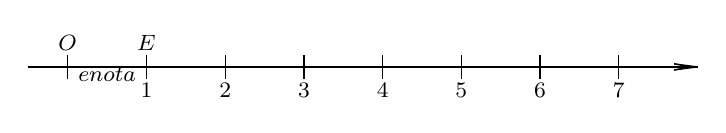
\begin{tikzpicture}
        % \clip (0,0) rectangle (14.000000,10.000000);
        {\footnotesize
        
        % Drawing segment a b
        \draw [line width=0.016cm] (0.500000,0.500000) -- (9.000000,0.500000);%
        
        % Drawing arrow a b 1.00
        \draw [line width=0.016cm] (8.702567,0.539158) -- (9.000000,0.500000);%
        \draw [line width=0.016cm] (8.702567,0.539158) -- (8.900856,0.500000);%
        \draw [line width=0.016cm] (8.702567,0.460842) -- (9.000000,0.500000);%
        \draw [line width=0.016cm] (8.702567,0.460842) -- (8.900856,0.500000);%
        
        % Drawing segment c d
        \draw [line width=0.016cm] (1.000000,0.350000) -- (1.000000,0.650000);%
        
        % Drawing segment e f
        \draw [line width=0.016cm] (2.000000,0.350000) -- (2.000000,0.650000);%
        
        % Drawing segment g h
        \draw [line width=0.016cm] (3.000000,0.350000) -- (3.000000,0.650000);%
        
        % Drawing segment i j
        \draw [line width=0.016cm] (4.000000,0.350000) -- (4.000000,0.650000);%
        
        % Drawing segment k l
        \draw [line width=0.016cm] (5.000000,0.350000) -- (5.000000,0.650000);%
        
        % Drawing segment m n
        \draw [line width=0.016cm] (6.000000,0.350000) -- (6.000000,0.650000);%
        
        % Drawing segment o p
        \draw [line width=0.016cm] (7.000000,0.350000) -- (7.000000,0.650000);%
        
        % Drawing segment r s
        \draw [line width=0.016cm] (8.000000,0.350000) -- (8.000000,0.650000);%
        
        % Marking point O
        \draw (1.000000,0.600000) node [anchor=south] { $O$ };%
        
        % Marking point E
        \draw (2.000000,0.600000) node [anchor=south] { $E$ };%
        
        % Marking point 1
        \draw (2.000000,0.400000) node [anchor=north] { $1$ };%
        
        % Marking point 2
        \draw (3.000000,0.400000) node [anchor=north] { $2$ };%
        
        % Marking point 3
        \draw (4.000000,0.400000) node [anchor=north] { $3$ };%
        
        % Marking point 4
        \draw (5.000000,0.400000) node [anchor=north] { $4$ };%
        
        % Marking point 5
        \draw (6.000000,0.400000) node [anchor=north] { $5$ };%
        
        % Marking point 6
        \draw (7.000000,0.400000) node [anchor=north] { $6$ };%
        
        % Marking point 7
        \draw (8.000000,0.400000) node [anchor=north] { $7$ };%
        
        % Marking point {enota}
        \draw (1.500000,0.600000) node [anchor=north] { ${enota}$ };%
        }
    \end{tikzpicture}
        
\end{figure}




Vsako število zapišemo s \textbf{številko}. 
Za zapis številke uporabljamo \textbf{števke}. Te so $0, 1, 2, 3, 4, 5, 6, 7, 8, 9$.



Posamezne števke večmestnega števila od desne proti levi predstavljajo: \textbf{enice}, \textbf{desetice}, \textbf{stotice}, \textbf{tisočice}, ...


~\newline
Število, ki je zapisano s črkovnimi oznakami števk označimo s črto nad zapsiom črkovne oznake.
$$ \overline{xy}=10x+y \quad \quad \quad \overline{xyz}=100x+10y+z$$




\end{priprava}